\documentclass[pdftex,12pt,a4paper]{article}

\usepackage[turkish,english]{}
\usepackage{graphicx}  
\usepackage[margin=2.5cm]{geometry}
\usepackage{breakcites}
\usepackage{indentfirst}
\usepackage{pgfgantt}
\usepackage{pdflscape}
\usepackage{float}
\usepackage{epsfig}
\usepackage{epstopdf}
\usepackage[cmex10]{amsmath}
\usepackage{url}
\usepackage{stfloats}
\usepackage{multirow}

\renewcommand{\refname}{REFERENCES}
\linespread{1.3}

\usepackage{mathtools}
%\newcommand{\HRule}{\rule{\linewidth}{0.5mm}}
\thispagestyle{empty}
\begin{document}
\begin{titlepage}
\begin{center}
\textbf{}\\
\textbf{\Large{ISTANBUL TECHNICAL UNIVERSITY}}\\
\vspace{0.5cm}
\textbf{\Large{COMPUTER ENGINEERING DEPARTMENT}}\\
\vspace{2cm}
\textbf{\Large{BLG 242E\\ LOGIC CIRCUITS LABORATORY\\ EXPERIMENT REPORT}}\\
\vspace{2.8cm}
\begin{table}[ht]
\centering
\Large{
\begin{tabular}{lcl}
\textbf{EXPERIMENT NO}  & : & 1 \\
\textbf{EXPERIMENT DATE}  & : & 14.02.2020 \\
\textbf{LAB SESSION}  & : & FRIDAY - 10.30 \\
\textbf{GROUP NO}  & : & 6 \\
\end{tabular}}
\end{table}
\vspace{1cm}
\textbf{\Large{GROUP MEMBERS:}}\\
\begin{table}[ht]
\centering
\Large{
\begin{tabular}{rcl}
{
150170706  & : & \c{S}AM\.{I}L TANER CENG\.{I}Z \\
150160514  & : & HAL\.{I}L \.{I}BRAH\.{I}M YAVUZ \\
150180251  & : & AHMET HAMZA KAYA \\
}
\end{tabular}}
\end{table}
\vspace{2.8cm}
\textbf{\Large{SPRING 2020}}

\end{center}

\end{titlepage}

\newpage

\thispagestyle{empty}
\addtocontents{toc}{\contentsline {section}{\numberline {}FRONT COVER}{}}
\addtocontents{toc}{\contentsline {section}{\numberline {}CONTENTS}{}}
\setcounter{tocdepth}{4}
\tableofcontents
\clearpage

\setcounter{page}{1}
\section{INTRODUCTION }

\begin{flushleft}
\paragraph{}
In this experiment, we used the axioms and theorems in Boolean Algebra and observed them using physical components on the CADET.
\end{flushleft}
\section{REQUIREMENTS}

\begin{flushleft}
\underline{Tools Used}
\end{flushleft}
\begin{itemize}
    \item C.A.D.E.T
    \item 74000 series ICs
    \begin{itemize}
        \item 74x$x^{1}$04 - Hex Inverter
        \item 74x$x^{1}$08 - Quadruple 2-input Positive AND Gates
        \item 74x$x^{1}$32 - Quadruple 2-input Positive OR Gates
    \end{itemize}
\end{itemize}

\begin{flushleft}
\section{EXPERIMENTS}
\subsection{PART 1}
\end{flushleft}

\begin{flushleft}
\paragraph{}
We designed the following circuits and connected the output cable to the LED to observe the actual output, we drew the circuits in Logisim and outputs support each other in both Logisim and CADET.
\end{flushleft}
\begin{figure}[H]
    \centering
    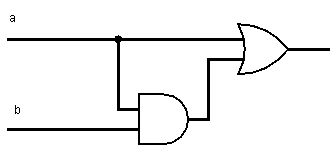
\includegraphics[width=0.5\textwidth]{circuit_1-1.png}
	\caption{circuit drawn with Logisim for a + a · b}
    \label{fig1}
\end{figure}
\begin{figure}[H]
    \centering
    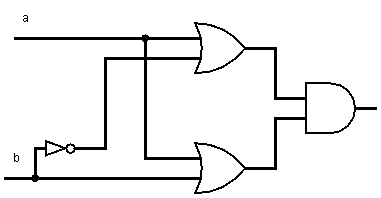
\includegraphics[width=0.5\textwidth]{circuit_1-2.png}
	\caption{circuit drawn with Logisim for (a+b).(a+b')}
	\label{fig2}
\end{figure}
\begin{flushleft} %second part
\paragraph{}
After creating the truth tables belonging to the circuit designs, we proved the design after observing that both circuits produce the same output in response to their corresponding  a and b input values.
\end{flushleft}
\begin{figure}[H]
    \centering
    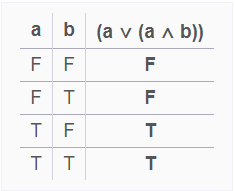
\includegraphics[width=0.5\textwidth]{table_1-1.png}
	\caption{truth table for  a+(a·b)}
    \label{tbl1}
\end{figure}

\begin{figure}[H]
    \centering
    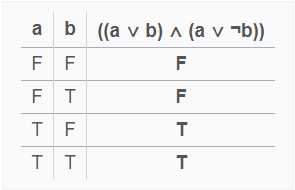
\includegraphics[width=0.5\textwidth]{table_1-2.png}
	\caption{truth table (a+b).(a+b')}
	\label{tbl2}
\end{figure}


\begin{flushleft}
\subsection{PART 2}
\end{flushleft}

\begin{flushleft} %fist part
\paragraph{}
In this part we proved that if a theorem is true it must be valid for both the current function and its dual. We observed the outputs of both original function and its dual to prove.
\end{flushleft}
\begin{figure}[H]
    \centering
    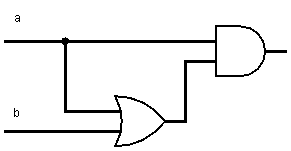
\includegraphics[width=0.5\textwidth]{circuit_2-1.png}
	\caption{circuit drawn with Logisim for a.(a+b)}
	\label{fig3}
\end{figure}


\begin{figure}[H]
    \centering
    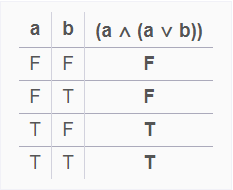
\includegraphics[width=0.5\textwidth]{table_2-1.png}
	\caption{truth table for a.(a+b)}
	\label{tbl3}
\end{figure}




\begin{flushleft}
\subsection{PART 3}
\end{flushleft}
\begin{flushleft}
\paragraph{}
Firstly, we found the complement of the given function then  we implemented both the function and its complement on the CADET.
\end{flushleft}

\begin{figure}[H]
    \centering
	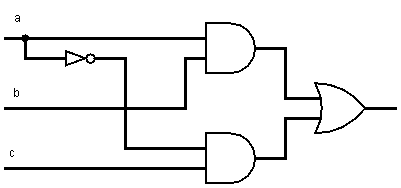
\includegraphics[width=0.5\textwidth]{circuit_3-1.png}
	\caption{circuit drawn with Logisim for F}
	\label{fig4}
\end{figure}
\begin{figure}[H]
    \centering
	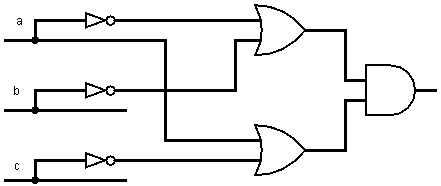
\includegraphics[width=0.5\textwidth]{circuit_3-2.png}
	\caption{circuit drawn with Logisim for F'}
	\label{fig5}
\end{figure}

\begin{flushleft} %second part
\paragraph{}
Afterwards, we observed the output on the LED then we compare the results with the outputs on the truth table and then we proved that the complement of the  function "F"  gives opposite output values for the same input values
\end{flushleft}
\begin{figure}[H]
    \centering
	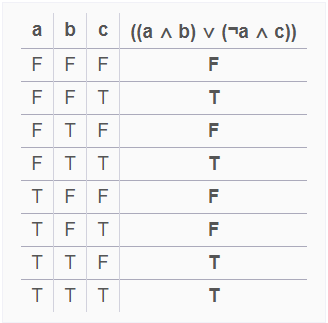
\includegraphics[width=0.5\textwidth]{table_3-1.png}
	\caption{truth table for F}
	\label{tbl4}
\end{figure}
\begin{figure}[H]
    \centering
	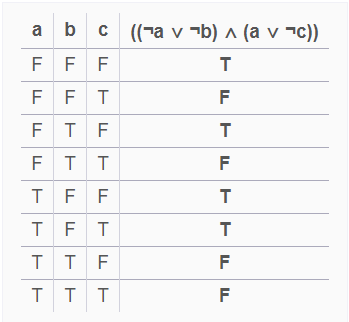
\includegraphics[width=0.5\textwidth]{table_3-2.png}
	\caption{truth table for F'}
	\label{tbl5}
\end{figure}

\begin{flushleft}
\subsection{PART 4}
\end{flushleft}

\paragraph{}
\begin{flushleft}
Initially we minimized the given function with using Karnaugh Map and implemented the minimized circuit on the Cadet. We got the simplified function as (c'.d)+(c.d'). Then, we realized that the minimized function can also be implemented using XOR gate.
\end{flushleft}
\begin{figure}[H]
    \centering
	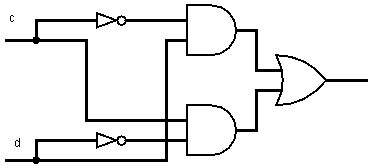
\includegraphics[width=0.5\textwidth]{circuit_4-1.png}
	\caption{circuit drawn with Logisim for (c'.d)+(c.d') }
	\label{fig6}
\end{figure}
\begin{figure}[H]
    \centering
	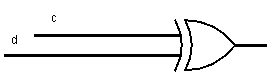
\includegraphics[width=0.5\textwidth]{circuit_4-2.png}
	\caption{(c'.d)+(c.d') with XOR gate}
	\label{fig7}
\end{figure}
\begin{flushleft} %second part
\paragraph{}
We observed the results and compared them with the truth table values (Important Note: Since the minimized function depends only on the c and d values and will be the same as the output value of the initially given function, the truth table was created by looking at only the c and d values).
\end{flushleft}
\begin{figure}[H]
    \centering
	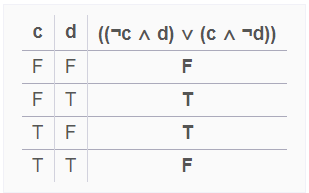
\includegraphics[width=0.5\textwidth]{table_4-1.png}
	\caption{truth table for (c'.d)+(c.d')}
	\label{tbl6}
\end{figure}






\section{DISCUSSION}
\begin{flushleft}
\paragraph{}
We can say that we remembered the axioms and theorems of Boolean algebra and how they work. We had the chance to implement some basic circuits which we covered in lectures from past period. Additionally, this experiment is a general introduction to Boolean algebra and we covered duality principle, de morgan law, karnough maps, truth tables and simplification processes.  we consolidate our knowledge about Boolean algebra with this experiment.

\end{flushleft}

\section{CONCLUSION}
We did not encounter any major difficulties except for one subject. In the experiment in the Part 1, we realized that we had a visual confusion while analyzing the circuit after we finished installing the circuit without paying attention to the color of the wires for each input. For this reason, we assigned  different colors for each input in the other parts, so we learned that we can easily analyze the circuit since we use wire of the same color for the same input.
\begin{flushleft}
\paragraph{}


\end{flushleft}



\newpage
\addcontentsline{toc}{section}{\numberline {}REFERENCES}
\nocite{ref1}
\nocite{report_guide}
\nocite{beginner_overleaf}

\bibliographystyle{unsrt}
\bibliography{reference}

\end{document}
